%\begin{tikzpicture} [   node distance = 1.7cm,
%                        on grid,
%                        state/.style={circle,inner sep=2pt}]
% 
%    % Help grid
%    %\draw [help lines] (-2,2) grid (2,-2);
%     
%    % States
%    \node[black, draw=white] (p)       [state]                     {\textbf{P}};
%    \node[black, draw=white] (np)      [state, above right = of p] {\textbf{NP}$ = \Sigma_1^p$};
%    \node[black, draw=white] (conp)    [state, below right = of p] {\textbf{coNP}$ = \Pi_1^p$};
%    \node[black, draw=white] (sigma2)  [state, right = of np]      {$\Sigma_2^p$};
%    \node[black, draw=white] (pi2)     [state, right = of conp]    {$\Pi_2^p$};
%    \node[black, draw=white] (sigma3)  [state, right = of sigma2]  {$\Sigma_3^p$};
%    \node[black, draw=white] (pi3)     [state, right = of pi2]     {$\Pi_3^p$};
%    \node[black, draw=white] (sigmai)  [state, right = of sigma3]  {$\Sigma_i^p$};
%    \node[black, draw=white] (pii)     [state, right = of pi3]     {$\Pi_i^p$};
%    \node[black, draw=white] (sigmai1) [state, right = of sigmai]  {$\Sigma_{i+1}^p$};
%    \node[black, draw=white] (pii1)    [state, right = of pii]     {$\Pi_{i+1}^p$};
%
%    \path [-stealth, thick]
%        (p) edge [] node {} (np)
%        (p) edge [] node {} (conp)
%        (np) edge [] node {} (sigma2)
%        (np) edge [] node {} (pi2)
%        (conp) edge [] node {} (sigma2)
%        (conp) edge [] node {} (pi2);
%        (sigma2) edge [] node {} (sigma3)
%        (sigma2) edge [] node {} (pi3)
%        (pi2) edge [] node {} (sigma3)
%        (pi2) edge [] node {} (pi3)
%        (sigmai) edge [] node {} (sigmai1)
%        (sigmai) edge [] node {} (pii1)
%        (pii) edge [] node {} (sigmai1)
%        (pii) edge [] node {} (pii1);
        %(sigma2) edge [] node {} (sigma3)
        %(sigma2) edge [] node {} (sigma3)
        %(sigma2) edge [] node {} (sigma3)
        %(sigma2) edge [] node {} (sigma3)
        %(sigma2) edge [] node {} (sigma3)
        %(sigma2) edge [] node {} (sigma3);
     
%\end{tikzpicture}

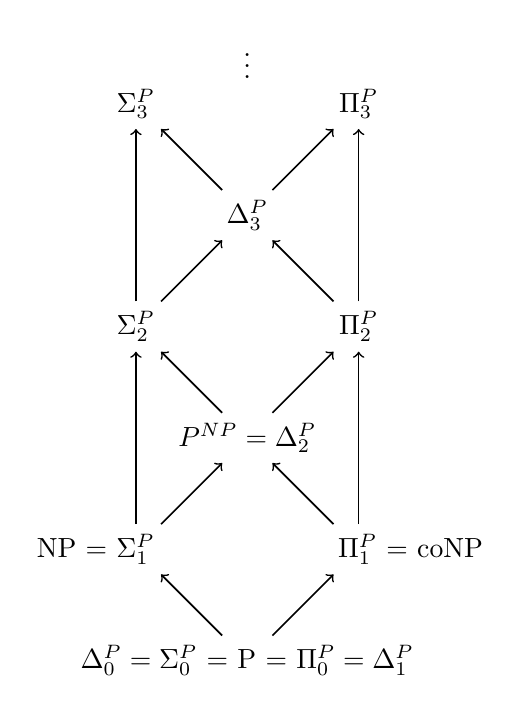
\begin{tikzpicture}[->, node distance=2cm, semithick]
    \node (P) {$\Delta_0^\text{P} =\Sigma_0^\text{P}$ = P = $\Pi_0^\text{P} = \Delta_1^\text{P}$};
    \node (Sigma1) [above left of=P]       {NP = $\Sigma_1^\text{P}$ \hspace*{0.9cm}};
    \node (Pi1)    [above right of=P]      {\hspace*{1.2cm} $\Pi_1^\text{P}$ = coNP};
    \node (Delta2) [above left of=Pi1]     {$\text{P}^\text{NP} = \Delta_2^\text{P}$};
    \node (Sigma2) [above left of=Delta2]  {$\Sigma_2^\text{P}$};
    \node (Pi2)    [above right of=Delta2] {$\Pi_2^\text{P}$};
    \node (Delta3) [above left of=Pi2]     {$\Delta_3^\text{P}$};
    \node (Sigma3) [above left of=Delta3]  {$\Sigma_3^\text{P}$};
    \node (Pi3)    [above right of=Delta3] {$\Pi_3^\text{P}$};
    \node (dots)   [above of=Delta3]       {\vdots};
    \draw (P)      -> (Sigma1);
    \draw (P)      -> (Pi1);
    \draw (Sigma1) -> (Sigma2);
    \draw (Sigma1) -> (Delta2);
    \draw (Pi1)    -> (Pi2);
    \draw (Pi1)    -> (Delta2);
    \draw (Delta2) -> (Sigma2);
    \draw (Delta2) -> (Pi2);
    \draw (Sigma2) -> (Sigma3);
    \draw (Sigma2) -> (Delta3);
    \draw (Pi2)    -> (Pi3);
    \draw (Pi2)    -> (Delta3);
    \draw (Delta3) -> (Sigma3);
    \draw (Delta3) -> (Pi3);
\end{tikzpicture}